$\chapter{Hausdorff Topological Spaces}



The following is a section of the great book ``Mathematical Discovery'' by Bruckner.
\begin{quote}
	Professional mathematicians must adhere to strict standards in their work. This entails providing precise definitions, even for seemingly familiar concepts. Such precision often requires the use of complex technical tools and methods. A mathematician must possess a clear understanding of fundamental concepts, such as the precise definition of a "curve," the mathematical interpretation of "traversing a curve with the inside to the left," the formal description of the number of "holes" in a pretzel, and the mathematical definition of area.
	
	\textbf{	It's important to note that this level of rigor and precision is not typically present when a mathematician initially approaches a problem and begins working on a solution.} In the early stages, ideas tend to be more abstract and intuitive. The refinement and meticulousness become evident only in the final drafts of mathematical work.
\end{quote}

Thus, we first need to have a discussion that show that the ideas behind the abstractions and generalizations are achievable by careful studying the mathematical objects already around us. This this section focuses to motivate the reader towards the more abstract concepts.

Thus we will discuss that the $\R^n$ along with the Euclidean distance has some special properties (which later will be generalized to the concept of metric spaces), and then we will see that the notion of Euclidean distance give rise to special sets called open ball which will give rise to the notion of open sets. We will study the properties of these open sets and later we will study what if we define the notion of open sets on its own (without any need to any particular metric) which will lead to the notions and ides of topological spaces. 

\section{Motivation}
Consider the set $\R^k$ which is a $k$ fold Cartesian product of our favorite set $\R$!. We can also extend the notion of Euclidean distance in $\R$ (which was simply $\abs{x-y}$ for $x,y\in\R$) to $\R^k$ as follows
\[ \abs{x-y} = \sqrt{\sum_{i=1}^{k} (y_i - x_i)^2}, \qquad x=(x_1,\cdots,x_k),\ y=(y_1,\cdots,y_k) \in \R^k. \]

We can easily observe that the Euclidean distance is a function $d:\R^k\times \R^k \to\R$ that satisfies the following properties
\begin{enumerate}[(i)]
	\item $\abs{x-y} \geq 0, \quad \abs{x-y}=0 \biImp x=y$,
	\item $\abs{x-y} = \abs{y-x}$,
	\item $\abs{x-y} \leq \abs{x-z} + \abs{z-y}$
\end{enumerate}
Later, We will study the generalized idea of such functions defined on a set which will give rise to the concept of metric spaces.

Now, we intuitively define the notion of ``open ball'' centered at $x\in\R^k$ with radius $r\in\R$ as follows
\[ \ball{x}{r} = \{ y\in\R^k:\ \abs{x-y}<r \}. \]
Then we define a set $A\subseteq\R^k$ to be a open set such that for every element $x\in\A$, we can have an open ball $\ball{x}{r}$ for some $r\in\R$ which is contained in $A$. More formally we can write
\[ \forall x \in A,\ \exists r>0 \st x\in\ball{x}{r}\subseteq\R^k. \] 
Since this notion is a very central one (as we will find out later), for $\R^k$, we have the notion of the set of all open sets of $\R^k$, for which we write $\mathcal{T}$.
 
Then we can go a little bit beyond the immediate intuition and define the notion of the set of all neighborhoods of $x$ as
\[ \mathcal{N}(x) = \{ S\subseteq \R^k:\ \exists u\in\mathcal{T},\ x\in u\subseteq S \} . \]
It immediately follows from the definition that all open balls containing $x$ (not necessarily containing $x$) are in $\mathcal{N}(x)$, along with other sets which satisfies the required property. We are now in a good shape to study the properties of the open sets $u\in\mathcal{T}$. We claim the followings are some of such properties (which as it will turn out are the central properties in some sense)
\begin{enumerate}[(i)]
	\item \[\emptyset,\ \R^k \in \mathcal{T}.\]
	\item \[\forall \mathcal{G} \subseteq \mathcal{T} \wh \bigcup_{g\in\mathcal{G}}g \in \mathcal{T}.\]
	\item \[ U_1,\cdots,U_n \in \mathcal{T},\ n\in\N \implies \bigcap_{i=1}^{n}U_i \in \mathcal{T}.\]
	\item \[ \forall x,y\in\R^k,\ \exists U,V \in \mathcal{T} \st x\in U,\ y\in V,\quad U\cap V = \emptyset. \]
\end{enumerate}


\begin{proof}
	TO BE ADDED.
\end{proof}

Since the notion of open sets is closely related with the distance function, thus there is no surprise that it can be used to express the ideas of convergence of a sequence in $\R^k$ (such a fundamental concept in analysis) with the new terminology. For instance, the following two statements are logically equivalent for $x_n\to\hat{x}$
\begin{enumerate}[(i)]
	\item $\forall \epsilon>0,\ \exists N>0,\st \forall n>N \wh \abs{x_n-\hat{x}} < \epsilon$.
	\item $\forall S \in \mathcal{N}(\hat{x}),\ \exists N>0,\st \forall n > N \wh x_n \in S$.
\end{enumerate}
\begin{proof}
	TO BE ADDED.
\end{proof}

\section{Metric Spaces}
Although $\R^k$ is a very useful set synthesized in a special way to meet most of our requirements (for instance the completeness arguments in the sense of Cauchy sequence, least upper bound property, and etc.) but not every set we encounter is $\R^k$. We can have sets that are globally very different than the ``\emph{flat}'' $\R^k$, for instance $\mathbb{S}^1$ (unit circle), $\mathbb{S}^1 \times \mathbb{S}^1$ (a tours), etc. One of the main approaches in dealing with such structures is to ``locally'' convert it  (in a useful way) to a collection (or atlas) of subsets of $\R^k$ and then work with the original ``alien'' set in an indirect way by focusing on these local images in $\R^k$. Apart from this approach, it is also useful to generalize the notions of distance in a set, which will enable us working with other classes of abstract structures without relying on $\R^k$, as some of them are way larger than $\R^k$. For instance, consider the set of all bounded function $f:[0,1]\to\R$. This set has a cardinality that is bigger than the cardinality of continuum. Also, might want to work with sets that are discrete in nature, like $\N$ which their cardinality is less than $\R^k$. So relying on $\R^k$ for all purposes is not feasible, thus it might be a good idea to have the notion of distance between elements in set.

\begin{definition}[Metric Space]
	A metric space is simply $(X,d)$ in which $X$ is a  set and $d:X\times X \to \R$ is a function called metric that satisfies the following properties
	
	\begin{enumerate}[(i)]
		\item $d(x,y) \geq 0,\quad d(x,y) =0 \biImp x=y$.
		\item $d(x,y) = d(y,x)$.
		\item $d(x,y) \leq d(x,z) + d(z,y)$.
	\end{enumerate}
	In which $x,y,z\in X$. 
\end{definition}
Now we can easily see that all of the notions like open balls, open sets, and etc. which we defined for $\R^k$ can also be defined for a metric space. We can define different metrics on a particular set based on our demands. In fact there are infinitely many ways to come up with a metric function. \textbf{One of our main tasks in studying metric spaces is to show that there are some properties of a metric space that are independent of a particular defined metric}. As we will see later, this will give rise to more abstract construct called topological spaces. 

\begin{definition}[Open Ball in $\R^k$]
	Let $(X,d)$ be a metric space. An open ball centered at $x\in X$ with radius $r$ is the set
	\[ \ball{r}{x} = \{ y\in X: d(y,x)<r \}, \]
\end{definition}


\begin{definition}[Open Set in $\R^k$]
	Let $(X,d)$ be a metric space and let $U\subseteq X$. $U$ is open if 
	\[ \forall x\in X,\ \exists \ball{r}{x} \st \ball{r}{x} \subseteq U. \]
	We denote the set of all open sets of $X$ as $\mathcal{T}$.
\end{definition}

A very useful intuition about open sets is that we can move around any points of the set (sufficiently small) and still be in the set. In other words, we can perturb the points of an open set (a sufficiently small perturbation) and still remain in the set. 

\begin{definition}[Neighborhood of $x$]
	Let $(X,d)$ be a metric space. Then the set of all neighborhoods of $x$ is
	\[ \mathcal{N}(x) = \{ S \in \mathcal{P}(X):\ \exists U \in \mathcal{T} \st x\in U \subseteq S\}. \]
	In other words, A neighborhood of $x\in X$, is the collection of all subsets of $X$, such that contains an open set containing $x$.
\end{definition}

\begin{remark}
	An open ball is an open set. This is not a tautological statement. The word ``open'' in the notion of open ball, has nothing to do with the word ``open'' in the notion of open set. however, we can show that an open ball is indeed an open set, thus deserves the name ``open''. In more accurate language 
	\begin{quote}
		Let $\hat{x}\in X,\ \hat{r}\in\R,\ \text{and define } U=\ball{\hat{r}}{\hat{x}}$. Then $U$ is an open set.
	\end{quote}
\end{remark}
\begin{proof}
	The proof of remark above can be facilitated by considering the following diagram.

	\begin{figure}[h!]
	\centering
	
	
	
	
	
	\tikzset{every picture/.style={line width=0.75pt}} %set default line width to 0.75pt        
	
	\begin{tikzpicture}[x=0.75pt,y=0.75pt,yscale=-1,xscale=1]
		%uncomment if require: \path (0,300); %set diagram left start at 0, and has height of 300
		
		%Shape: Arc [id:dp8474273111700028] 
		\draw  [draw opacity=0][dash pattern={on 4.5pt off 4.5pt}] (237.52,62.7) .. controls (251.49,54.62) and (267.7,50) .. (285,50) .. controls (337.47,50) and (380,92.53) .. (380,145) .. controls (380,161.12) and (375.99,176.3) .. (368.9,189.59) -- (285,145) -- cycle ; \draw  [dash pattern={on 4.5pt off 4.5pt}] (237.52,62.7) .. controls (251.49,54.62) and (267.7,50) .. (285,50) .. controls (337.47,50) and (380,92.53) .. (380,145) .. controls (380,161.12) and (375.99,176.3) .. (368.9,189.59) ;  
		%Shape: Circle [id:dp7267488539784774] 
		\draw  [fill={rgb, 255:red, 65; green, 117; blue, 5 }  ,fill opacity=1 ] (280,140.3) .. controls (280,139.03) and (281.03,138) .. (282.3,138) .. controls (283.57,138) and (284.6,139.03) .. (284.6,140.3) .. controls (284.6,141.57) and (283.57,142.6) .. (282.3,142.6) .. controls (281.03,142.6) and (280,141.57) .. (280,140.3) -- cycle ;
		%Shape: Circle [id:dp26539586062898435] 
		\draw  [fill={rgb, 255:red, 65; green, 117; blue, 5 }  ,fill opacity=1 ] (340,112.3) .. controls (340,111.03) and (341.03,110) .. (342.3,110) .. controls (343.57,110) and (344.6,111.03) .. (344.6,112.3) .. controls (344.6,113.57) and (343.57,114.6) .. (342.3,114.6) .. controls (341.03,114.6) and (340,113.57) .. (340,112.3) -- cycle ;
		%Shape: Circle [id:dp3683519373366817] 
		\draw  [dash pattern={on 4.5pt off 4.5pt}] (319.13,112.3) .. controls (319.13,99.5) and (329.5,89.13) .. (342.3,89.13) .. controls (355.1,89.13) and (365.48,99.5) .. (365.48,112.3) .. controls (365.48,125.1) and (355.1,135.48) .. (342.3,135.48) .. controls (329.5,135.48) and (319.13,125.1) .. (319.13,112.3) -- cycle ;
		%Shape: Circle [id:dp20369737869678683] 
		\draw  [fill={rgb, 255:red, 65; green, 117; blue, 5 }  ,fill opacity=1 ] (335.4,97.7) .. controls (335.4,96.43) and (336.43,95.4) .. (337.7,95.4) .. controls (338.97,95.4) and (340,96.43) .. (340,97.7) .. controls (340,98.97) and (338.97,100) .. (337.7,100) .. controls (336.43,100) and (335.4,98.97) .. (335.4,97.7) -- cycle ;
		
		% Text Node
		\draw (268,138) node [anchor=north west][inner sep=0.75pt]  [font=\scriptsize] [align=left] {$\displaystyle \hat{x}$};
		% Text Node
		\draw (347,106) node [anchor=north west][inner sep=0.75pt]  [font=\scriptsize] [align=left] {$\displaystyle x$};
		% Text Node
		\draw (196,34) node [anchor=north west][inner sep=0.75pt]  [font=\scriptsize] [align=left] {$\displaystyle U=\mathcal{B}_{\hat{r}}(\hat{x})$};
		% Text Node
		\draw (349,136) node [anchor=north west][inner sep=0.75pt]  [font=\scriptsize] [align=left] {$\displaystyle \mathcal{B}_{\epsilon }( x)$};
		% Text Node
		\draw (340,91) node [anchor=north west][inner sep=0.75pt]  [font=\scriptsize] [align=left] {$\displaystyle \mu $};
		
		
	\end{tikzpicture}
\end{figure}
	
	Considering the visual idea, we can proceed with the proof. Let $x\in U$. Then let $r^* = r - d(x,\hat{x})$ and $\epsilon < r^*$. This implies that $d(x,\hat{x})=\hat{r}-r^*$. We claim that $\ball{\epsilon}{x} \subseteq U$. Indeed, let $\mu \in \ball{\epsilon}{x} $. By definition $d(\mu,x)<\epsilon<r^*$. Thus
	\[ d(\hat{x},\mu) \leq d(\hat{x},x) + d(x,\mu) < (\hat{r}-r^*) + r^* = \hat{r}. \]
	Thus we showed that $\mu \in \ball{\epsilon}{x}$ implies $\mu \in \ball{\hat{r}}{\hat{x}}$. Thus we can conclude that $\ball{\epsilon}{x} \subseteq \ball{\hat{r}}{\hat{x}}$, for any choice of $x$. Thus $U$ is an open set. 
\end{proof}

Following our arguments in the motivation section, we argued that the open sets of $\R^k$ satisfy some properties. If you read the proof closely, we used no facts very special about the Euclidean distance other than the properties described in the definition of a metric space. Thus it is not a surprise if we observe that those properties also hold for a general metric space. 

\begin{proposition}
	Let $(X,d)$ be a metric space. Then the open sets determined by $d$ satisfy the following properties
	\begin{enumerate}[(i)]
		\item $X,\emptyset \in \mathcal{T}$.
		\item $\mathcal{G}\subseteq \mathcal{T} \implies \bigcup_{g\in\mathcal{G}} g \in \mathcal{T}$.
		\item $U_1,\hdots,U_n \in \mathcal{T} \implies \bigcap_{i=1}^{n}U_i \in \mathcal{T}$.
		\item $\forall x,y\in X,\ \exists U,V \in \mathcal{T} \st x\in U,\ y\in\ V,\ U\cap V = \emptyset$.
	\end{enumerate}
\end{proposition}
\begin{proof}
	TO BE ADDED.
\end{proof}


The metric spaces can be very abstract, like the space of all functions with a suitable metric indeed forms a metric space. However, this space is infinite dimensional and its cardinality is even larger than the cardinality of continuum. However, following the following definition we can decide if certain subsets of those abstract spaces are bounded or not.
\begin{definition}[Bounded sets in a metric space]
	Let $(X,d)$ be a metric space and $A \subseteq X$. Then $A$ is bounded, if there exist $R \in \R$ and $x \in X$ such that $X \subseteq \ball{R}{x}$
\end{definition}


Also, one interesting fact about the metric space, is that, no matter what is the nature of metric space, the union of all cocentric ball with natural numbers as their radius, centered at any point of the metric space covers the whole space. The following proposition makes this more formal.

\begin{proposition}
	\label{prop:CocentericBallsCoveringMetricSpace}
	Let $(X,d)$ be a metric space and $x \in X$. Then for 
	\[ \mathcal{G} = \{ \ball{r}{x}: r \in \N \}, \]
	we have
	\[ X = \bigcup \mathcal{G}. \]
\end{proposition}
\begin{proof}
	Let $y \in X$. Then $d(x,y) = R$ for some $R \in \R$. Since $\exists N \in \N$ such that $R < N$, then $y \in \ball{n}{x}$ for all $n \geq N$. As for the converse, let $x \in \bigcup \mathcal{G}$. Then trivially $x \in X$. This completes the proof.
\end{proof}

\autoref{prop:CocentericBallsCoveringMetricSpace} is a very interesting result. It is somehow fascinating that every metric space can be covered with countable number of cocentric open balls. 


\begin{remark}
	One thing that the reader might note is the construct called ``long line'' which is a topological space which is longer than the real line in some sense. The long line consists of an uncountable number of copies of $[0,1)$ ``pasted together'' end-to-end. This is a topological space and not a metric space. Thus out argument remains valid
\end{remark} 


\subsection{Convergence in Metric Spaces}
So far, we only hand the notion of sequence in sets like $\R,\Z,\Q$, etc. and we developed the notion of convergence of a sequence by $\epsilon-N$ business. Remember that a sequence is a fundamental concept which enables us to discover the word which could be reached via the infinitely long road of sequences! For a detailed discussion see my opinion piece titled by ``What the Hell is Analysis?''. Now, the beauty of metric spaces is that we can analyze sequences in abstract metric spaces. This is automatically done via the structure of the metric function as for any pair $(x,y)\in X\times X$ it returns a real number which carries some intuitive information about the closeness of the points. So the if sequence $\{x_n\}$ whose elements live in $X$, converge to $\hat{x}\in X$, then this fact is basically translates to a bunch of real numbers approaching $0$ which can be easily analyzed using numerous tools we have already developed (like the squeeze theorem, etc.)

For instance, in finding the solution of a particular ordinary differential equation, we can can come up with an iteration process (which is known as contraction mapping) which acts on the space of function. Then we can prove that the trajectory of points created by repeated application of the map on some initial point, will converge (in the sense that the distance between the output $n$th iteration of the map on the initial point and the point that it converges to is getting closed to zero). This leads to the well-known ``Picard-Lindelöf'' theorem which states that under some conditions, an initial value problem has unique solution.

\begin{definition}
	Let $(X,d)$ be a metric space. Then the sequence $\seq{x}$ converges to $\hat{x}\in X$ if
	\[ \forall \epsilon>0,\ \exists N>0:\ \forall n>N \wh d(x_n,\hat{x})<\epsilon\ (\equiv  x_n \in \ball{\epsilon}{\hat{x}}) \]
	Or alternatively, using the notion of Neighborhood
	\[ \forall S \in \mathcal{N}(\hat{x}),\ \exists N>0:\ \forall n>N \wh x_n \in S.  \]
\end{definition}

We can show that these two definitions are in fact equivalent by following argument
\begin{proof}
	Since the statements (a) and (b) are equivalent, then we need to proof the both ways. Both proofs are straight and can be deduced by following the definitions.
	\begin{itemize}
		\item (a)$\implies$(b): Given $S\in \mathcal{N}(\hat{x}),\ \exists \ball{r}{\bar{x}}$ for $r>0$ sufficiently small. Let $r=\epsilon$. Since (a) is true, then $\exists N>0$ such that $\forall n>N$ we have $x_n \in \ball{\epsilon}{\hat{x}} \subseteq S$.
		\item (b)$\implies$(a): Given $\epsilon>0$, let $S = \ball{\epsilon}{\hat{x}}$. Then since (b) is true, then $\exists N>0$ suc that $\forall n>N$ we have $x_n \in S$, thus we conclude $x_n \in \ball{\epsilon}{\hat{x}}$. 
	\end{itemize}
\end{proof}


Another interesting fact to consider about the metric spaces is the interplay between sequences and open sets. This interplay is important since the notion of sequences and converges is tightly bound with the notion of metric in a metric space. On the other hand, although the open sets are actually generated by the metric, but, as we will see later, they can have their own world, meaning that we can define then as sets that satisfy some basic axiom. Thus any useful interplay between sequences and converges between open sets can be useful in the future generalizations.

The following proposition defines the notion of open sets in a metric space (which we originally define by the notion of open balls) using the idea of sequences and their convergence. 

\begin{proposition}
	In a metric space $(X,d)$, with subset $A$, the following are equivalent:
	\begin{enumerate}[(a)]
		\item $A$ is an open set.
		\item For every $x\in A$, and every sequence $\seq{x}$ obeying $x_n\to x$, one has $x_n\in A$ for all $n$ sufficiently large. That is 
		\[ \exists N \in \N:\ \forall n>N,\ x_n \in A. \]
	\end{enumerate}
\end{proposition}


\begin{proof}
	\begin{itemize}
		\item $(a) \implies (b)$: We assume that $A$ is open. Then for $x\in A$, we can pick a $\ball{\epsilon}{x} \subseteq A$ for some $\epsilon>0$. Then from the definition of convergence, we know that if $x_n \to x$, then $\exists N>0$ such that $\forall n>N$ we have $x_n \in \ball{\epsilon}{x}$ thus $x_n\in A$.
		
		\item $(b) \implies (a)$: We can prove this by both direct proof and also by contrapositive statement. For the direct proof, the idea is to consider the set of all sequences $x_n \to \x$ for $x\in A$. Then for each such sequence we can find $N>0$, such that $\forall n>N$ we have $x_n \in A$. We pick $x_{N+1}$ from all of such sequences and construct a set S such that $d(x,x_{N+1})\in S$. We let $r$ be the infimum of $S$. Infimum exists (since $S\subseteq \R$) and is nonzero (otherwise we could come up with a sequence that falsifies the assumption). We let $B = \ball{r}{x}$. Due to the construction $B \subseteq A$, thus implies $A$ is an open set. 
		
		However, the proof by contrapositive is much more straight forward. Assume $a$ is not true. Then for a given $n \in \N$, let $\epsilon=1/n$. Then since $A$ is not open then $\exists x\in A$ such that  $\ball{\epsilon}{x} \cap A \neq \emptyset$. Pick any $y \in \ball{\epsilon}{x} \cap A \neq$ and call it $x_n$. Due to the construction, $x_n \to x$, while $\forall n\in\N,\ x_n\notin A$ which implies $b$ is not true as well. 
		
	\end{itemize}
\end{proof}


\section{Completeness of Metric Spaces}

First we start with the notion of Cauchy sequences.
\begin{definition}[Cauchy sequences]
	Let $(X,d)$ be a metric space and $\seq{x}$ a sequence in $X$. Then $\seq{x}$ is Cauchy if 
	\[  \forall \epsilon > 0:\ \exists N>0 \st \forall n,m > N \wh d(x_n, x_m) < \epsilon.  \]
\end{definition}

And then we have the following very important definition.

\begin{definition}[Complete metric space]
	Let $(X,d)$ be a metric space. This space is complete, if every Cauchy sequence has a limit in $X$.
\end{definition}

The following proposition lists some of the important and basic properties of Cauchy sequences.

\begin{proposition}
	Let $(X,d)$ be a metric space. Then 
	\begin{enumerate}[(i)]
		\item Every converging sequence is Cauchy.
		\item Every Cauchy sequence is bounded.
		\item Every closed subset of a complete metric space, is complete.
		\item If a Cauchy sequence $\seq{x}$ has a converging sub-sequence that converges to some point $\hat{x}$, then the full original Cauchy sequence must converge to $\hat{x}$.
		\item Every compact metric space is complete.
	\end{enumerate}
\end{proposition}

\begin{proof}
	The proof for different items are as follows.
	\begin{enumerate}[(i)]
		\item Assume $\epsilon>0$ is given and $\{x_n\}$ converges to $\hat{x} \in K$. From the properties of metric function we have
		\[ d(x_n, x_m) \leq d(x_n,\hat{x}) + d(x_m,\hat{x}). \]
		Since $\seq{x}$ converges, then $\exists N_1 > 0$ such that $\forall n > N_1$ we have $d(x_n,\hat{x}) < \epsilon/2$. So for $n,m > N$ we have
		\[  d(x_n, x_m) \leq d(x_n,\hat{x}) + d(x_m,\hat{x}) < \epsilon,\]
		thus $\seq{x}$ is Cauchy. \qed
		
		\item Fix $\epsilon=1$. Then since $\seq{x}$ is Cauchy, then $\exists N > 0$ such that $d(x_N, x_m) < 1 $ for all $m > N$. Let
		\[ \hat{R} = \{ d(x_N, x_n):\ n < N, n \in \N \}. \]
		Let $ R = \max\set{1,\hat{R}}$. Thus due the the construction we have
		\[ x_n \in \ball{R}{x_N}, \quad \forall n \in \N. \]
		This completes the proof. \qed
		
		\item Let $\seq{x}$ be a Cauchy sequence in $F$. Thus $A = \{x_n:\ n\in\N \} \subseteq F \subseteq X$. Since $\seq{x}$ is also at $X$, then it converges to $\hat{x}\in X$. From definition of limit point (or derived set) we have $\hat{x} \in A'$. On the other hand $A \subseteq F \biImp A' \subseteq F'$. Since $F$ is closed, then $F' \subseteq F$. This implies $A' \subseteq F$. Thus $\hat{x} \in F$. This shows that $F$ is complete.    \qed
		
		\item Let $x_{n_k}$ be the converging sub-sequence, i.e. $x_{n_k} \to \hat{x}$ as $k \to \infty$. For a given $\epsilon$, since $\seq{x}$ is Cauchy, then $\exists N_1 > 0$ such that $\forall n,n_k > N_1$ we have $d(x_n, x_{n_k})<\epsilon/2$. Also, since $\{x_{n_k}\}$ is converging to $\hat{x}$, then $\exists N_2 > 0$ such that $\forall n_k, n_l > N_2$ we have $d(x_{n_l}, x_{n_k}) < \epsilon/2$. Let $N = \max\set{N_1,N_2}$. Then $\forall n > N$ (also $n_k > N$) we have
		\[ d(x_n, \hat{x}) \leq d(x_n, x_{n_k}) + d(x_{n_k},\hat{x}) < \epsilon/2 + \epsilon/2 = \epsilon.\]
 		Thus the original sequence converges to $\hat{x}$. \qed
 		
 		\item Every compact metric space is sequentially compact (see \autoref{thm:SequencialCompactness}), thus every sequence has a convergent sub-sequence that converges to a point in the metric space. Let $\seq{x}$ be a Cauchy sequence. This will have a converging sub-sequence that converges to a point in $\hat{x} \in X$. But as we showed in (iv), this sequence itself converges to $\hat{x}$. Thus $X$ is complete.
	\end{enumerate}
\end{proof}

The following proposition is a very important one that has numerous use cases in the filed of functional analysis.

\begin{proposition}
	For any non-empty set $S$, let $M(S)$ denote the set of all bounded real-valued functions on S. In symbols we have
	\[ M(S) = \{ f:S\to \R\ :\ \sup_{x\in S}\abs{f(x)}< \infty \}. \]
	define $d: M(S)\times M(S) \to \R$ as 
	\[ d(f,g)= \sup_{x\in S}\abs{f(x)-g(x)}. \]
	The $(M(S),d)$ is a \textbf{complete metric space.}
\end{proposition}

\begin{proof}
	First we need to show that this is actually a metric space, i.e. the function $d$ satisfies the metric properties. --> TOBE ADDED
	
	For the second part, which is more important, is to show that this metric space is actually complete. To show this, let $\seq{f}$ be a Cauchy sequence in $M(S)$. Thus from definition we have
	\[ \forall \epsilon >0,\ \exists N>0\:\ \forall n,m>N \wh \sup_{x\in S}\abs{f_n(x)-f_m(x)} < \epsilon. \]
	From the definition of suprimum (least upper bound), we can conclude that
	\[ \forall x\in S \wh \abs{f_n(x) - f_m(x)} < \epsilon. \]
	This means that for every $x\in S$ the sequence $f_n(x)$ forms a Cauchy sequence in $\R$, thus it converges to some value, say $\hat{f}(x)$. We claim that the Cauchy sequence $\seq{f}$ converges to $\hat{f}$. To show this we need to first show that $\hat{f} \in M(S)$ and the show that $f_n \to \hat{f}$.
	
	To show $\hat{f} \in M(S)$ we seek help from an special function $\textbf{0}$ which assigns the value $0 \in \R$ to every $x\in S$. Since $\seq{f}$ is Cauchy, then it is bounded, thus $\exists R > 0$ such that $f_n \in \ball{R}{\textbf{0}}$ for all $n \in \N$. Using the definition of open ball we can write
	\[ \sup_{x\in S}\abs{f_n(x) - \textbf{0}(x)} = \sup_{x\in S}\abs{f_n(x)} < R. \]
	From the definition of $\sup$ we can conclude that 
	\[ \forall x\in S,\ \forall n\in \N \wh f_n(x) < R. \]
	By $n\to \infty$ we can write
	\[ \forall x\in S \wh \hat{f}(x) < R \implies \sup_{x\in S}\abs{\hat{f}(x)} \leq R. \]
	This shows that $\hat{f} \in M(S)$.
	
	To show that $f_n \to \hat{f}$, let $\epsilon>0$ be given. Then since for every $x\in A$ the sequence $f_n(x)$ converges to $\hat{f}(x)$ we can fine $N_x \in \N$ such that $\forall n > N_x$ we have $\abs{f_n(x) - \hat{f}(x)} < \epsilon/2$. Let $N = \sup\{N_x\}$. We know that $N < +\infty$ since otherwise it means that there exists $N_x$ for some $x\in A$ that is larger than any real number, which contradicts the fact that $f_n(x)$ converges to $\hat{f}(x)$. Now $\forall n>N_x$ we have
	\[ \forall x\in S:\ \abs{f_n(x) - \hat{f}(x)} < \epsilon/2. \]
	This implies
	\[ \sup_{x\in S} \abs{f_n(x) - \hat{f}(x)} \leq \epsilon/2 < \epsilon. \]
	Thus $f \to \hat{f}$, and this completes the proof.
\end{proof}


\section{Hausdorff Topological Spaces}
Metric spaces are natural extensions to the idea of $R^k$ along with the Euclidean distance function. However, we can go even further, and show that some notions we encountered before are really independent of a particular metric. All such arguments are under the umbrella of topological spaces. 

\begin{definition}
	A topological space has two arguments: A set $X$, and a family $\mathcal{T}$ of subsets of $X$ called ``the open sets'', that have the following properties. 
	\begin{enumerate}[(i)]
		\item Both $\emptyset$ and $X$ are in $\mathcal{T}$.
		\item Any union of open sets is open. That is for any subset $\mathcal{G} \subseteq \mathcal{T}$ one has $\bigcap \mathcal{G} \in \mathcal{T}$.
		\item Any intersection of \textbf{finitely many} open sets is open. That is if $N\in \N$ and $U_1, \cdots, U_n \in \mathcal{T}$, then $U_1 \cap \cdots \cap U_n \in \mathcal{T}$.
	\end{enumerate}
\end{definition}

Given the definition above, we can now have the following important remark. 


\begin{remark}
	In a nutshell, a metric space is a topological space whose opens sets are determined by the notion of open balls. The following diagram summarizes this fact.
	\begin{center}

	
	
	\tikzset{every picture/.style={line width=0.75pt}} %set default line width to 0.75pt        
	
	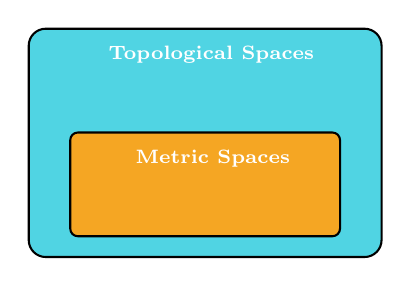
\begin{tikzpicture}[x=0.75pt,y=0.75pt,yscale=-1,xscale=1]
		%uncomment if require: \path (0,300); %set diagram left start at 0, and has height of 300
		
		%Rounded Rect [id:dp8983262620207249] 
		\draw  [fill={rgb, 255:red, 80; green, 212; blue, 227 }  ,fill opacity=1 ] (80,78.2) .. controls (80,73.67) and (83.67,70) .. (88.2,70) -- (241.8,70) .. controls (246.33,70) and (250,73.67) .. (250,78.2) -- (250,171.8) .. controls (250,176.33) and (246.33,180) .. (241.8,180) -- (88.2,180) .. controls (83.67,180) and (80,176.33) .. (80,171.8) -- cycle ;
		%Rounded Rect [id:dp4318601497382968] 
		\draw  [fill={rgb, 255:red, 245; green, 166; blue, 35 }  ,fill opacity=1 ] (100,123.73) .. controls (100,121.67) and (101.67,120) .. (103.73,120) -- (226.27,120) .. controls (228.33,120) and (230,121.67) .. (230,123.73) -- (230,166.27) .. controls (230,168.33) and (228.33,170) .. (226.27,170) -- (103.73,170) .. controls (101.67,170) and (100,168.33) .. (100,166.27) -- cycle ;
		
		% Text Node
		\draw (117,77) node [anchor=north west][inner sep=0.75pt]  [font=\scriptsize] [align=left] {\textcolor[rgb]{1,1,1}{\textbf{Topological Spaces}}};
		% Text Node
		\draw (130,127) node [anchor=north west][inner sep=0.75pt]  [font=\scriptsize,color={rgb, 255:red, 255; green, 255; blue, 255 }  ,opacity=1 ] [align=left] {\textbf{Metric Spaces}};
		
		
	\end{tikzpicture}
\end{center}
\end{remark}

So from now on, all of our definitions and proofs will be in a topological setting. The following example illustrates some topological spaces.

\begin{itemize}
	\item Discrete topology: For any $X$ let $\mathcal{T} = \mathcal{P}(X)$. Then any subset of $X$ will be an open set.
	\item Trivial topology: For any $X$ let $\mathcal{T} = \{ \emptyset, X \}$.
	\item The usual topology on $\R^k$: Let $X = \R^k$. Let $U \in \mathcal{T}$ if $\forall x\in U$ there exists $\ball{\epsilon}{x} \subseteq U$ for some $\epsilon>0$.
	\item Sorgenfrey line: Let $X= \R$. Then $G\subseteq \R$ belongs to $\mathcal{T}$ if and only if $\forall x\in G$, there exists $r>0$ such that $[x,x+r) \subseteq G$.
	\item Let $X = \{1,2,3\}$ and $\mathcal{T}=\{ \{1,2\}, \{1,3\}, \{1\}, \{1,2,3\},\emptyset \}$. This is an example of non-Hausdorff topology, where there are not enough open sets available to isolate some points of the set via disjoint open sets. For instance, there are not disjoint open sets in $U,V \in \mathcal{T}$ such that $1\in U$ and $2\in V$. The following figure represents the configuration of the open sets.
	\begin{figure}[h!]
	\centering
	
	
	\tikzset{every picture/.style={line width=0.75pt}} %set default line width to 0.75pt        
	
	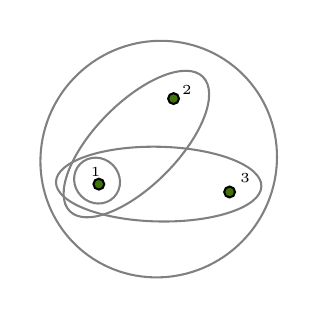
\begin{tikzpicture}[x=0.75pt,y=0.75pt,yscale=-0.9,xscale=0.9]
		%uncomment if require: \path (0,300); %set diagram left start at 0, and has height of 300
		
		%Shape: Circle [id:dp6254924747106434] 
		\draw  [fill={rgb, 255:red, 65; green, 117; blue, 5 }  ,fill opacity=1 ] (180,132.9) .. controls (180,131.3) and (181.3,130) .. (182.9,130) .. controls (184.5,130) and (185.8,131.3) .. (185.8,132.9) .. controls (185.8,134.5) and (184.5,135.8) .. (182.9,135.8) .. controls (181.3,135.8) and (180,134.5) .. (180,132.9) -- cycle ;
		%Shape: Circle [id:dp48431322085787665] 
		\draw  [fill={rgb, 255:red, 65; green, 117; blue, 5 }  ,fill opacity=1 ] (250,137.1) .. controls (250,135.5) and (251.3,134.2) .. (252.9,134.2) .. controls (254.5,134.2) and (255.8,135.5) .. (255.8,137.1) .. controls (255.8,138.7) and (254.5,140) .. (252.9,140) .. controls (251.3,140) and (250,138.7) .. (250,137.1) -- cycle ;
		%Shape: Circle [id:dp35320390948185487] 
		\draw  [fill={rgb, 255:red, 65; green, 117; blue, 5 }  ,fill opacity=1 ] (220,87.1) .. controls (220,85.5) and (221.3,84.2) .. (222.9,84.2) .. controls (224.5,84.2) and (225.8,85.5) .. (225.8,87.1) .. controls (225.8,88.7) and (224.5,90) .. (222.9,90) .. controls (221.3,90) and (220,88.7) .. (220,87.1) -- cycle ;
		%Shape: Ellipse [id:dp6827777295590995] 
		\draw  [color={rgb, 255:red, 128; green, 128; blue, 128 }  ,draw opacity=1 ] (167.37,147.4) .. controls (158.67,138.78) and (167.57,115.69) .. (187.24,95.83) .. controls (206.91,75.96) and (229.91,66.84) .. (238.61,75.46) .. controls (247.3,84.07) and (238.41,107.16) .. (218.74,127.02) .. controls (199.07,146.89) and (176.07,156.01) .. (167.37,147.4) -- cycle ;
		%Shape: Ellipse [id:dp2922418509608795] 
		\draw  [color={rgb, 255:red, 128; green, 128; blue, 128 }  ,draw opacity=1 ] (159.96,131.71) .. controls (160.2,120.67) and (185,112.24) .. (215.36,112.88) .. controls (245.73,113.53) and (270.15,123.01) .. (269.91,134.05) .. controls (269.68,145.09) and (244.87,153.52) .. (214.51,152.87) .. controls (184.15,152.23) and (159.73,142.75) .. (159.96,131.71) -- cycle ;
		%Shape: Ellipse [id:dp2556128273268483] 
		\draw  [color={rgb, 255:red, 128; green, 128; blue, 128 }  ,draw opacity=1 ] (173.59,139.43) .. controls (168.61,134.5) and (168.32,126.73) .. (172.93,122.07) .. controls (177.55,117.41) and (185.32,117.63) .. (190.3,122.55) .. controls (195.28,127.48) and (195.57,135.26) .. (190.96,139.92) .. controls (186.34,144.58) and (178.57,144.36) .. (173.59,139.43) -- cycle ;
		%Shape: Ellipse [id:dp36749477614063886] 
		\draw  [color={rgb, 255:red, 128; green, 128; blue, 128 }  ,draw opacity=1 ] (169.98,164.9) .. controls (145.36,140.52) and (145.53,100.42) .. (170.37,75.34) .. controls (195.21,50.26) and (235.3,49.69) .. (259.92,74.07) .. controls (284.54,98.45) and (284.36,138.55) .. (259.53,163.63) .. controls (234.69,188.71) and (194.6,189.28) .. (169.98,164.9) -- cycle ;
		
		% Text Node
		\draw (177,122.4) node [anchor=north west][inner sep=0.75pt]  [font=\tiny]  {$1$};
		% Text Node
		\draw (225.8,78.4) node [anchor=north west][inner sep=0.75pt]  [font=\tiny]  {$2$};
		% Text Node
		\draw (257,125.6) node [anchor=north west][inner sep=0.75pt]  [font=\tiny]  {$3$};
		
		
	\end{tikzpicture}
\end{figure}
\end{itemize}





\subsection{Neighborhoods and Interior Points}
\begin{definition}
	Let $(X,\mathcal{T})$ be a topological space. Then for $x\in X$, we write $\mathcal{N}(x)$ to denote the set of all neighborhoods of $x$ defined as 
	\[ \mathcal{N}(x) = \{ S \subset X:\ \exists u\in\mathcal{T} \st x\in u \subseteq S \}. \]
\end{definition}
Every open set containing $x\in X$ belongs to $\mathcal{N}(x)$. Often, some non-open sets do, too.

\begin{lemma}{}
	Let $(X, \mathcal{T})$ be a topological space. Then the following are equivalent
	\begin{enumerate}[(a)]
		\item $A \in \mathcal{T}$.
		\item $\forall x\in A \wh A \in \mathcal{N}(x)$.
	\end{enumerate}
\end{lemma}
\begin{proof} The proof is as follows: 
	\begin{itemize}
		\item $(a) \implies (b)$: Since $A$ is open, then trivially, for $x\in A$ we have $x\in A \subseteq A$. Thus following the definition of $\mathcal{N}(x)$ we conclude that $A \in  \mathcal{N}(x)$.
		\item $(b) \implies (a)$: Let $x \in A$. Then from $(b)$ we know that $A \in  \mathcal{N}(x)$. Thus $\exists U_x \in \mathcal{T}$ such that $x\in U_x \subseteq A$. Then construct the set $\mathcal{G}$ as 
		\[ \mathcal{G} = \bigcup_{x\in A} U_x. \]
		From definition of open sets, $\mathcal{G}$ is open as it is union open sets. Also $x \in \mathcal{G}$ then $\exists U_x \subseteq A$, thus $\mathcal{G} \subseteq A$. On the other hand, $x\in A$ then $x\in U_x \subseteq \mathcal{G}$, thus $A \subseteq \mathcal{G}$, So we conclude $A = \mathcal{G}$.
	\end{itemize}
\end{proof}

The beautiful fact about topological spaces is that since they contain the metric spaces as a special case, then it means that we can generalize the ideas of ``interior'', ``boundary'', etc. using purely topological arguments.

\begin{definition}
	Let $A$ be any set in a topological space $(X,\mathcal{T})$. The set of interior points of $A$ are defined as
	\[ A^{\circ} = \{ x\in A:\ \exists U\in \mathcal{T} \st x\in U \subseteq A \}. \]
\end{definition}

\begin{corollary}
	Let $(X,\mathcal{T})$ be a topological space and $A,B \subseteq X$. Then 
	\[ A \subseteq B \implies A^\circ \subseteq B^\circ. \]
\end{corollary}
\begin{proof}
	This corollary follows immediately from the definition. Let $x\in A^\circ$. Then $\exists U \in \mathcal{T}$ such that $x\in U \subseteq A \subseteq B$. Then $x \in B^\circ$ as well.   
\end{proof}

The corollary above, somehow give the intuition, that $A^\circ$ is in some sense, the largest open set contained in $A$.


\begin{proposition}
	Let $(X,\mathcal{T})$ be a topological space and $A$ any set in $X$. Then 
	\begin{enumerate}[(a)]
		\item $A^\circ$ is open, and $A^\circ \subseteq A$.
		\item If $G$ is open and $G \subseteq A$, then $G \subseteq A^\circ$.
		\item $A$ is open if and only if $A = A^\circ$.
	\end{enumerate}
\end{proposition}
\begin{proof}
	The proof for different parts of the proposition are as follows
	\begin{enumerate}[(a)]
		\item Let $x\in A^\circ$. To show that $A^\circ$ is open it is enough to show that $A^\circ \in \mathcal{N}(x)$. From definition of an interior point, $\exists U \in \mathcal{T}$ such that $x\in U \subseteq A$. Now $\forall z\in U$ we have $z\in U \subseteq A$, thus $z\in A^\circ$, implying $U\subseteq A^\circ$, thus $A^\circ \in \mathcal{N}(x)$. So $A^\circ$ is an open set (following from the lemma we proved above). Furthermore, $A^\circ \subseteq A$ follows immediately from definition. Let $x\in A^\circ$. Then $\exists U \in \mathcal{T}$ such that $x \in U \subseteq A$ thus $A^\circ \subseteq A$.
		\item Since $G \in \mathcal{T}$, and $G\subseteq A$, then $\forall x\in G$ we have $x\in G \subseteq A$, thus $x \in A^\circ$. This implies $G \subseteq A^\circ$.
		
		\item This proof will have two parts. Part 1: $A$ is open $\implies A = A^\circ$. Then we can write
		\begin{align*}
			& x \in A \implies x \in A \subseteq A \implies x \in A^\circ \implies A \subseteq A^\circ. \\
			& x \in A^\circ \implies \exists U \in \mathcal{T}: x \in U \subseteq A \implies A^\circ \subseteq A.
		\end{align*} 
		Thus we can conclude that $A = A^\circ$. For the converse, we need to prove $A=A^\circ$ implies $A$ is open. One of the important tools for this purpose is the lemma we proved before. To show that $A$ is open we need to show that it is a Neighborhood of all of its elements (i.e. contains an open set which contains that point). More formally, let $x\in A$. Since $A = A^\circ$, then $x \in A^\circ$, Thus $\exists U \in \mathcal{T}$ such that $x \in U \subseteq A$. This implies that $A \in \mathcal{N}(x)$. thus we can conclude that $A$ is an open set.
	\end{enumerate}
\end{proof}


\section{Closed sets and Closure}
The interplay between true and false statements in logic, in which the latter is the negation of the former, leads to concepts like ``De Morgan's'' law. Because of this particular law, we have the dual concept of open sets, which we know as closed sets. There is nothing special about open sets that the notion of closed sets lack. They both are two sides of a single thing. So, we can actually build the whole concepts of topology out of closed sets.

\begin{definition}
	Let $(X,\mathcal{T})$ be a topological space. Then $A \subseteq X$ is a closed set if and only if it complement $A^c$ is an open set. 
\end{definition}

Note that the notion of closed set is \textbf{not} the negation of open sets. Thus we can have sets that are both open and closed, while we can have sets that are neither open not closed. For instance, in every topological space, the sets $\emptyset$ and $X$ are always both open and closed (sometimes called clopen sets).

\begin{lemma}{}
	Let $(X,\mathcal{T})$ be a topological space with $A \subseteq X$. Then the following two statements are equivalent.
	\begin{enumerate}[(a)]
		\item $A$ is closed.
		\item For every $x \notin A$, $\exists U \in \mathcal{N}(x)$ such that $U \subseteq A^c$.
	\end{enumerate}
\end{lemma}
\begin{proof}
	The proof will have two sections as follows:
	\begin{itemize}
		\item $(a) \implies (b)$: Since $A$ is closed, then $A^c$ is open, thus it is a neighborhood of all of its elements. So $\forall x\in A^c,\ \exists U \in \mathcal{T}$ such that $x \in U \subseteq A^c$.
		\item $(b) \implies (a)$: $\forall x \in A^c,\ \exists U \in \mathcal{N}(x)$ such that $x\in U \subseteq A^c$. Since $U \in \mathcal{N}(x)$, then $\exists V \in \mathcal{T}$ such that $x\in V \subseteq U \subseteq A^c$. Thus we conclude that $A^c \in \mathcal{N}(x)$. This implies that $A^c$ is open, hence $A$ is closed. 
	\end{itemize}
\end{proof}

\begin{proposition}
	Let $(X,\mathcal{T})$ be a topological space. Then 
	\begin{enumerate}[(a)]
		\item Any intersection of closed sets is closed.
		\item Finite union of closed sets is closed.
	\end{enumerate}
\end{proposition}
\begin{proof}
	The De Morgan's law play a central role in the proof.
	\begin{enumerate}[(a)]
		\item Let $F$ be a set of closed sets. Then 
		\[ (\bigcap F)^c = (\bigcup F^c) \]
		is open as it is union of open sets (i.e. $F^c$). This implies that $\bigcap F$ is closed. 
		\item Let $F = \{F_1, \cdots, \F_n\}$ be a collection of closed sets. Then 
		\[ (\bigcup_{i=1}^{n} F_i)^c = \bigcap_{i=1}^n F_i^c \]
		is open (as it is finite intersection of open sets. Thus $\bigcup_{i=1}^{n} F_i$ is closed.
	\end{enumerate}
\end{proof}

\begin{definition}
	Let $(X,\mathcal{T})$ be a topological space with $A \subseteq X$. Then the closure of $A$ is defined as
	\[ \overline{A} = ((A^c)^\circ)^c \]
\end{definition}

From the definition, we can conclude the following corollary
\begin{corollary}
	Let $(X,\mathcal{T})$ be a topological space with $A,B \subseteq X$. Then we have
	\[ A \subseteq B \implies \overline{A} \subseteq \overline{B} \]
\end{corollary}
\begin{proof}
	We can prove the statement following some basic set operations
	\[ A \subseteq B \implies A^c \supseteq B^c \implies (A^c)^\circ \supseteq (B^c)^\circ \implies ((A^c)^\circ)^c \subseteq ((B^c)^\circ)^c. \]
\end{proof}

There is a very beautiful parallel between the notions of interior of a set and the closure of a set. For instance, the closure of a set, is the smallest closed set containing the original set. The parallel interior points and the closure is very similar to the parallel between infimum (biggest lower bound) and supremum (least upper bound).

\begin{proposition}
	\begin{enumerate}[(a)]
		\item $\overline{A}$ is closed and $A \subseteq \overline{A}$
		\item If $F$ is closed and $A \subseteq F$, then $\overline{A} \subseteq F$.
		\item $A$ is closed if and only if $A = \overline{A}$.
	\end{enumerate}
\end{proposition}

\begin{proof} The proof for each statement is as follows:
	\begin{enumerate}[(a)]
		\item From definition, the closure of a set is a compliment of an open set (complement of $(A^c)^\circ$). Thus it is closed by definition. Further more, let $x\in A$. Then $x\notin A^c \implies x\notin (A^c)^\circ$. Thus $x \in ((A^c)^\circ)^c$, hence $A \subseteq \overline{A}$. Also, we can present this proof in a different way as follows
		\[ (A^c)^\circ \subseteq A^c \implies ((A^c)^\circ)^c \supseteq A. \]
		\item Since $F$ is closed, then $F^\circ$ is open, and since it is open then $(F^c)^\circ = F^c$. Then we can write
		\[ A \subseteq F \implies A^c \supseteq F^c \implies (A^c)^\circ \supseteq F^c \implies ((A^c)^\circ)^c \subseteq F. \]
		\item This also follows immediately from the properties of open sets. For the first part, assume $A$ is closed. Then $A^c$ is open, and is the same as its interior, i.e. $(A^c)^\circ = A^c$. Computing the complements of both sides will result in $((A^c)^\circ)^c = A$, thus $\overline{A} = A$. As for the converse, Assume $A = \overline{A}$. Thus from definition $A = ((A^c)^\circ)^c$. Then $A^c = (A^c)^\circ$. This implies that $A^c$ is open, hence $A$ is closed. 
	\end{enumerate}
\end{proof}

\section{Boundary Points}
So far, we studied the notion of open sets that had some information about the interior of a set, and also we studied the notion of closed sets that has some information about the complement of a set. The notion of boundary of a set, kind of ties these two concepts to each other. In fact, as we will prove later, the boundary of a set, is the intersection of the closure of a set with the closure of its complement.
\begin{definition}
	Let $(X,\mathcal{T})$ be a topological space with $A \subseteq X$. Then $x\in X$ is a \emph{boundary point} of $A$ if 
	\[ \forall U\in \mathcal{T} \cap \mathcal{N}(x),\ U \cap A \neq \emptyset,\ U \cap A^c \neq \emptyset. \]
	The set of all boundary points of $A$ is denoted as $\partial A$. 
\end{definition}

Few points to easily digest the above definition. First, $U \in \mathcal{T} \cap \mathcal{N}(x)$ in words means $U$ is an open set containing $x$. Also, note that the boundary point of $A$ can be in $A$ or in $A^c$. Also, equivalently, we can express the definition as $x$ is a boundary point of $A$ if $\forall U\in \mathcal{N}(x),\ U \cap A \neq \emptyset,\ U \cap A^c \neq \emptyset$. 

\begin{corollary}
	Let $(X,\mathcal{T})$ be a topological space with $A \subseteq X$. Then 
	\[ \partial (A) = \partial (A^c). \]
\end{corollary}
\begin{proof}
	This follows immediately from the definition and the symmetrical appearance of $A$ and $A^c$ in the definition, such that interchanging their position does not matter.
\end{proof}

\begin{proposition}
	Let $(X,\mathcal{T})$ be a topological space. Then 
	\begin{enumerate}[(a)]
		\item $\partial A = \overline{A} \cap \overline{A^c}$.
		\item $A$ is closed if and only if $\partial A \subseteq A$; also, $\overline{A} = A \cup \partial A$.
		\item $A$ is open if and only if $\partial A \subseteq A^c$; also, $A^\circ = A \backslash \partial A$.
	\end{enumerate}
\end{proposition}

\begin{proof}
	The proof of each section is as follows:
	\begin{enumerate}[(a)]
		\item This proof has two sections. First we show that $\partial A \subseteq \overline{A} \cap \overline{A^c}$. We use the proof by contrapositive. Let $x\notin \overline{A} \cap \overline{A^c}$. Thus $x\notin ((A^c)^\circ)^c \cap (A^\circ)^c$. Then by De Morgan's law we have $x \in (A^c)^\circ \cap A^\circ$. This says that $x$ should be in the interior of $A$ or $A^c$, each of which implies that $x \notin \partial A$. That is because
		\begin{align*}
			& x \in (A^c)^\circ \implies \exists U \in \mathcal{T}:\ x\in U \subseteq A^c \implies A \notin \partial A\\
			& x \in A^\circ \implies \exists V \in \mathcal{T}:\ x\in V \subseteq A \implies A \notin \partial A.
		\end{align*}
		However for the converse, we show $x \notin \partial A$ leads to $x \notin \overline{A} \cap \overline{A^c}$ (i.e. contrapositive of the actual statement that we need to prove). Let $x \notin \partial A$. Then $\exists U \in \mathcal{N}(x)$ such that $U \cap A = \emptyset$ or $U \cap A^c = \emptyset$, each of which implies $x \notin \overline{A} \cap \overline{A^c}$. Indeed $U \cap A = \emptyset$ implies $x \notin \overline{A}$, thus $x \notin \closure{A} \cap \closure{A^c}$. Similarly $U \cap A^c = \emptyset$ implies $x \notin \closure{A^c}$, thus $x \notin \closure{A} \cap \closure{A^c}$.
		
		\item This proof has two sections. THIS PROOF TO BE COMPLETED. 
		\begin{itemize}
			\item For the first part, we want to show that $A$ is closed implies $\partial A \subseteq A$. For this purpose we can take very different ways, i.e. to use the the tools already developed (like the one we proved in section (a)), or to use the basic definitions. For instance to assume that we want to use the tool developed in part (a). Let $x \in \partial A$. So, from (a) we can write $x \in \closure{A}  \cap \closure{A^c} \biImp x \in ((A^c)^\circ)^c \cap (A^\circ)^c$. Since $A$ is closed, then $A^c$ is open. This implies that $A^c = (A^c)^\circ$. Thus $x \notin (A^c)^\circ \cup A^\circ \biImp  x \notin A^c \cap A^\circ \biImp x \in A \cap (A^\circ)^c$, thus $x \in A$. This concludes that $x \in A$, hence $\partial A \subseteq A.$
			
			However, we can take slightly  different approaches as well. Since $A$ is open, then $A^c$ is closed. To show $\partial A \subseteq A$ we can show by contrapositive i.e. $x\notin A \implies x \notin \partial A$. Since $x\notin A$, then $x \in A^c$, and since $A^c$ is open then $x \in (A^c)^\circ$. This implies $x \notin ((A^c)^\circ)^c$, thus $x \notin \closure{A}$. From (a), again, we can conclude that $x \notin \partial A$.
		\end{itemize}
		
	\end{enumerate}
\end{proof}



\section{Limit Points and Isolated Points}
The notion of a limit point is very important in a topological space, as it has a very intuitive sequential characterization in a metric space, and has a very interesting connection with other topological notions such as closed and open sets.

\begin{definition}
	Let $(X,\mathcal{T})$ be a topological space. A point $x \in X$ is a limit point of $A \subseteq X$ if 
	\[ \forall U \in \mathcal{N}(x), \wh (U\backslash\{x\}) \cap A \neq \emptyset.  \]
\end{definition}


\section{Sequential Characterization}
Naturally, we have the concept of sequences and limits of sequences in metric spaces. On the other hand, we studied that the topological spaces are generalized form of metric spaces. This means that all of topological concepts we covered so far (i.e. open sets, closed sets, interior points, closure, limit points, etc) can be characterized with the notion of a sequence and convergence in metric spaces. This is very important since sequences are some tools that are easier to conceive intuitively. 

The concept of limit point in the topological sense is easier to characterize sequentially, and then characterize other notions using the interplay between the limit point and those concepts. The following proposition reveals a very important characterization.


\begin{proposition}
	\label{sequential}
	In a metric space $(X,d)$ with $A \subseteq X$. the followings are equivalent
	\begin{enumerate}[(a)]
		\item $x$ is a limit point of $A$
		\item There exists a sequence $x_n$ with distinct elements such that $x_n \to x$.
	\end{enumerate}
\end{proposition}
\begin{proof}
	This proof will have two parts as follows.
	\begin{itemize}
		\item $(a) \implies (b)$. We assume that $x$ is a limit point of $A$ and we need to come up with a smartly designed sequence with distinct elements, all of which lies in $A$ such that $x_n \to x$. Since $x \in  A'$, then $\forall \mathbb{B}(x;r)$ for $r\in \R$ we have $\mathbb{B}(x;r) \cap A \neq \emptyset$. Let $r_1 = 1$. Choose $x_1 \in  \mathbb{B}(x;r_1) \cap A$. Let $r_2 = d(x_1,x)/2$ and choose $x_2 \in \mathbb{B}(x;r_2) \cap A$. Similarly, let $r_3 = d(x_2,x)/2$ and choose $x_3 \in \mathbb{B}(x;r_3) \cap A$, and we continue the construction. Then, due to the construction, all of the elements of $\seq{x}$ has distinct elements. Also since $d(x_n,x)\leq 2^{-n}$, then $x_n \to x$. This complete the proof.
		
		\item $(b) \implies (a)$. We assume that there is a sequence $\seq{x}$ with distinct elements in $A$ that approaches $x$. Let $S \in \mathcal{N}(x)$. The from definition there is a ball $\mathbb{B}[x;r)$ for some $r\in \R$ such that $\mathbb{B}[x;r) \subseteq S$. On the other hand, from the definition of convergence we know $\exists N>0$ such that $\forall n>N$ we have $x_n \in \mathbb{B}[x;r)$. Since $x_n$ has all distinct elements, then $\mathbb{B}[x;r)$ still contains $x_n$ excluding at most one element. Hence $S\backslash\{x\} \cap A \neq \emptyset$. Since $S$ was chosen arbitrary, then this is true for all $S \in \mathcal{N}(x)$. This completes the proof.
	\end{itemize} 
	
\end{proof}

We can have a similar approach and characterize the notion of isolated points with the notion of sequences in a metric space. Since the set of isolated points of $A$ is $A \backslash A'$, then we can have the following proposition.


\begin{proposition}
	Let $(X,d)$ be a metric space with $A \subseteq X$. Then $x \in A$ is an isolated point of $A$ is there are no sequence with distinct elements that approach $x$.
\end{proposition} 

\begin{proof}
	TO BE ADDED.
\end{proof}

One of the useful interplay between the notion of limit point and the notion of open sets is the following proposition.

\begin{proposition}
	Let $(X,\mathcal{T})$ be a topological space. Then
	\[ G \in \mathcal{T} \Longleftrightarrow G \cap (G^c)' = \emptyset, \]
	in which $(\cdot)'$ denotes the set of all limit points.
\end{proposition}

Using this interplay we can have a sequential characterization of the notion of open set.

\begin{proposition}[Sequential characterization of open sets]
	Let $(X,d)$ be a metric space. Then $A \subseteq X$ is open if and only there are no sequences approaching $x$ with distinct elements all of which lies in $A^c$.
\end{proposition}

As we saw before, the notion of boundary points is very crucial, since the notion of interior points and also closure of a set can be define using that (i.e. $A^\circ = A \backslash \partial A$ and $\closure{A}= A \cup \partial A$). The following proposition makes a connection between the notion of a boundary point in topological space and the notion of sequence and its limit in a metric space.

\begin{proposition}
	Let $(X,d)$ be a metric space. Then $x \in \partial A$ if and only if there exist two sequence $x_n$ and $y_n$ such that $x_n \to x$ and $y_n \to x$, and $x_n \in A,\ y_n \in A^c$ for all $n$ sufficiently large. 
\end{proposition}

\begin{proof}
	Let $x \in \partial A$. Since $(X,d)$ is a topological space, then $\forall \epsilon > 0,\ \exists \ball{\epsilon}{x}$ such that $\ball{\epsilon}{x} \cap A \neq \emptyset$ and $\ball{\epsilon}{x} \cap A^c \neq \emptyset$. We construct the sequences $\seq{x}$ and $\seq{y}$ with the following construction. For a given $n \in \N$, let $\epsilon=1/n$. Then pick $x_n \in \ball{\epsilon}{x} \cap A$ and $y_n \in \ball{\epsilon}{x} \cap A^c$. Due to the construction, we have $x_n\to x$ also $y_n \to x$ with the required property that $x_n \in A$ and $y_n \in A^c$ for all $n \in \N$.
\end{proof}


\subsection{Base of Topology}
The notion of the base of topology is a very useful and practical tool to analyze relatively complex topological spaces. The following is from the Wikipedia article about the notion  of bases of a topology
\begin{quote}
	Bases are ubiquitous throughout topology. The sets in a base for a topology, which are called \emph{basic open sets}, are often easier to describe and use than arbitrary open sets. Many important topological definitions such as \emph{continuity} and \emph{convergence} can be checked using only basic open sets instead of arbitrary open sets. Some topologies have a base of open sets with specific useful properties that may make checking such topological definitions easier.
	
	Not all families of subsets of a set \( X \) form a base for a topology on \( X \). Under some conditions detailed below, a family of subsets will form a base for a (unique) topology on \( X \), obtained by taking all possible unions of subfamilies. Such families of sets are very frequently used to define topologies. A weaker notion related to bases is that of a \emph{subbase} for a topology. Bases for topologies are also closely related to \emph{neighborhood bases}.
\end{quote}

There are many ways to interpret the idea of topological bases. Here, we will cover two of them.
\begin{definition}
	Let $(X,\mathcal{T})$ be a topological space. Then $\mathcal{B} \subseteq \mathcal{T}$ is a basis for topology if and only if $\forall U \in \mathcal{T}$ there exists $B \subseteq \mathcal{B}$ such that $\bigcup B = U$. 
\end{definition}

The definition above, focuses on an existing topological space with given $\mathcal{T}$. However, we can have a quite opposite point of view, with some flavors of reverse engineering. Consider the following proposition.

\begin{proposition}
	Let $X$ be a  non-empty set. Take a collection of subsets $\mathcal{B} \subseteq \mathcal{P}(X)$. Try using the sets in $\mathcal{B}$ to define the notion of neighborhood of $x\in X$ as follows
	\[ \mathcal{N}(x) = \{ S \subseteq x:\ \exists U \in \mathcal{B} \st x \in U \subseteq S \}. \]
	Then declare a set $G \subseteq X$ to be ``open'' if and only of $G \in \mathcal{N}(x)$ holds for all $x\in G$.
	
	The construction above, defines a Hausdorff topological space if $\mathcal{B}$ satisfies the following properties. 
	\begin{enumerate}[(a)]
		\item $\bigcap \mathcal{B} = X $ [i.e. every point in $X$ belongs to at least one set $B \in \mathcal{B}$].
		\item Whenever $B_1, B_2 \in \mathcal{B}$ and $x \in B_1 \cap B_2$, then there exists some $B \in \mathcal{B}$ such that $x \in B \subseteq B_1 \cap B_2$.
		\item $\forall x,y \in X$ we have $B_1, B_2 \in \mathcal{B}$ such that $x \in B_1$ and $x \in B_2$ while $B_1 \cap B_2 = \emptyset$.
	\end{enumerate} 

	Such a set $\mathcal{B}$ is called a base for $\mathcal{T}$.
\end{proposition}


\begin{proof}
	TO BE ADDED.
\end{proof}

\begin{example}
	Let $(\R, d)$ be a metric space in which $d$ is the Euclidean metric. This metric induces the notion of open balls in $(\R, d)$. Consider the set
	\[ \mathcal{B} = \{ \ball{\epsilon}{x}:\ \epsilon, x \in \Q \}. \]
	There are in fact balls which are centered at rational numbers and has rational radius. We can prove that this set is a basis for $(\R, \mathcal{T})$ in which $\mathcal{T}$ is the usual topology. We can show that via definition of basis (i.e. to show that every $U \in \mathcal{T}$) can be written as a union of subsets of $\mathcal{B}$, or, alternatively, we can show $\mathcal{B}$ is basis via showing that we can construct $\mathcal{T}$ via the construction discussed in the proposition above (which boils down to showing that $\mathcal{B}$ satisfies the required conditions).
	
	The basis $\mathcal{B}$ is interesting since it is countable. The topological spaces that admit a countable basis are called \emph{second-countable} spaces.  
\end{example}


\subsection{Summary}
Here in this section we are going to summarize all of the properties of topological spaces.

\begin{summary}[Open sets and the interior points]
	Let $(X,\mathcal{T})$ be a topological spaces. Then $A \in \mathcal{T}$ is called an open set and has the following properties
	\begin{itemize}
		\item $A$ is open if and only if $A = A^\circ$.
		\item $A$ is open if and only if $\forall x \in A \wh A \in \mathcal{N}(x)$.
		\item $A$ is open if and only if $A \cap (A^c)' = \emptyset$.
		\item $A^\circ = A \backslash \partial A$
	\end{itemize}
\end{summary}

\begin{summary}[Closed sets and the closure]
	Let $(X,\mathcal{T})$ be a topological space. Then
	\begin{itemize}
		\item $F$ is closed if and only if $F^c$ is open.
		\item $F$ is closed if and only if $F = \closure{F}$.
		\item $F$ is closed if and only if $F' \subseteq F$.
		\item $\closure{F} = F \cup \partial F$. 
	\end{itemize}
\end{summary}

\begin{summary}[Subset preserving operations!]
	Let $(X,\mathcal{T})$ be a topological space, and $A,B \subseteq X$. If $A \subseteq B$, then 
	\begin{itemize}
		\item $A^\circ \subseteq B^\circ$.
		\item $\closure{A} \subseteq \closure{B}$.
		\item $A' \subseteq B'$.
	\end{itemize}
\end{summary}


\section{Compactness}
We start with the definition of compactness.

\begin{definition}[Compactness]
	Let $(X,\mathcal{T})$ be a topological space. Then $K \subseteq X$ is compact, if for every collection of open sets $\mathcal{G} \subseteq \mathcal{T}$ satisfying $K \subseteq \bigcup_{G \in \mathcal{G}} G$ (which is called an open cover), we have a finite sub collection $\{ G_1, G_2, \cdots, G_N \}$ for some $N \in \N$ such that $K \subseteq \bigcup_{i=1}^N G_i$ (which is called a finite sub-cover).
	In words, a set is compact, if every open cover admits a finite sub-cover.
\end{definition}


\begin{remark}
	Compactness is the next best thing to finiteness. It's so valuable that when it is absent, we sometimes switch to a new topology in which compactness is present. 
\end{remark}

Furthermore, the notion of compactness is expressing the fact that if $K \subseteq X$ is compact, then we can find an open set $G$ that can be constructed via union of only finite ingredients in $\mathcal{T}$ and $K \subseteq G$.

\begin{lemma}
	Let $(X,\mathcal{T})$ be a topological space. Then $S \subseteq X$ finite, is a compact set.
\end{lemma}

\begin{proof}
	Let $\mathcal{G} \subseteq \mathcal{T}$ be an open cover for $S = \{x_1, \cdots, x_N\}$ for some $N \in \N$. Then since $S \subseteq \bigcap \mathcal{G}$, then each $x_i \in S$ belongs to some $G_i$ in $\mathcal{G}$. Then $\{G_1, \cdots, G_N \}$ is a sub-cover that is finite.
\end{proof}

\begin{lemma}
	Let $(\R, \abs{\cdot})$ be a metric space. Then $\Z \subseteq \R$ is not compact.
\end{lemma}

\begin{proof}
	To show $\Z \subseteq \R$ is not compact, we need to find an open cover that fails to have a finite sub-cover. Let $\mathcal{G} = \{ \ball{1/4}{x}: x\in \Z \}$. $\mathcal{G}$ is an open cover, but it fails to have any sub-cover. Since any $G \in \mathcal{G}$ covers only one integers, and for any choice of $N \in \N$ the sub-cover $H = \{ G_1, \cdots, G_N\}$ won't cover all of $\Z$. Thus $\Z$ is not compact. 
\end{proof}

The following is a very important proposition which helps in making some intuition about the compact sets.

\begin{proposition}
	Let $(X,d)$ be a metric space, and $K \subseteq X$ compact. Then $K$ is bounded.
\end{proposition}

\begin{proof}
	Let $x \in X$. Then from \autoref{prop:CocentericBallsCoveringMetricSpace} we define
	\[ \mathcal{G} =  \{ B_r(x): r \in \N \}, \]
	and we get $X = \bigcup \mathcal{G}$. Then $K \subseteq \mathcal{G}$. Thus $\mathcal{G}$ is an open cover. Since $\mathcal{K}$ is compact, then there is a finite sub-cover $ \mathcal{H} = \{ B_{r_1}(x), \cdots, B_{r_N}(x) \}$ for some $N \in \N$, such that $K \subseteq \bigcup \mathcal{H}$. Let $r = \max \{r_1, \cdots, r_N\}$ and $z \in K$. Then $\exists B_{r_i}(x) \in \mathcal{H}$ such that $z \in B_{r_i}(x) \subseteq B_r(x)$. Thus $K \subseteq B_r(x)$. This shows that $K$ is bounded. 
\end{proof}




\begin{lemma}
	In $(\R,\abs{\cdot})$, the set $S = \{1/n: n \in \N \}$ is not compact, but the set $\closure{S} = S \cup \{0\}$ is compact. 
\end{lemma}

\begin{proof}
	To show that $S$ is not compact, we can easily show that there is an open cover that fails to have a finite sub-cover. A great candidate for that is a family of open sets each of which contains only one $x \in S$. Consider 
	\[ \mathcal{G} = \{ \ball{r}{n}: n \in \N, r = 1/(n+1)^2 \}. \]
	This is an open cover all if its elements are open sets and $S \subseteq \mathcal{G}$. Since each element of $\mathcal{G}$ contains only one element of $S$, then $\mathcal{G}$ fails to have finite subset that covers $S$. Thus $S$ is not compact.
	
	The second part of proof is to show that $S \cup \closure{S}$ is compact. Let $\mathcal{G}$ be an open cover. Then there is an open set $G \in \mathcal{G}$ such that $0 \in G$. Since $G$ is open and contains 0, and also the sequence $\{1/n\}$ goes to 0, then $\exists N \in \N$ such that $\forall n > N$ we have $1/n \in G$. Thus $G$ contains all but finitely many elements of $S$. However for each $1/n$ with $1 \leq n \leq N$ we have $G_n \in \mathcal{G}$ such that contains $1/n$. Thus $\{ G, G_1, \cdots, G_N \}$ is a finite sub-cover, thus the set $S\cup \closure{S}$ is compact.
\end{proof}


\begin{remark}
	The proposition above can be extended to show that for any convergent sequence in any metric space, the closure of the range is compact.
\end{remark}

The following proposition is an important one, as it is true only in Hausdorff topological spaces, and not in general topological spaces.

\begin{proposition}
	\label{prop:CompactSetIsClosedHausdorff}
	Let $(X,\mathcal{T})$ be a \textbf{Hausdorff} topological space and $K \subseteq X$ compact. Then $K$ is closed. In other words, in any Hausdorff topological space, a compact set contains all of its limit points. 
\end{proposition}

\begin{proof}
	Since this proposition is only true for Hausdorff topological spaces, then we have the hint that we should use some properties specific to the Hausdorff topological spaces. We want to show that $K^c$ is open. Since an open set is a neighborhood of all of its elements, thus for $y \in K^c$ we need to find an open set $S$ such that $y \in S \subseteq K^c$.
	
	Let $y \in K^c$. Then since $\forall x \in K$, there exists $U_x, V_x \in \mathcal{T}$ such that $ x \in U_x$ and $y \in V_x$ and $U_x \cap V_x = \empty$. This is the same as writing $V_x \subseteq U_x^c$. Clearly, $\mathcal{G} = \{ U_x: x \in K \}$ is an open cover for $K$. But since $K$ is compact, then $\mathcal{G}$ admits an open sub-cover. Thus $\exists x_1, \cdots, x_N \in K$ for some $N \in \N$ such that $K \subseteq \bigcup_{i=1}^{N} U_{x_i}$. Then we can write
	\[ K^c \supseteq \bigcap_{i=1}^{N} U_{x_i}^c \supseteq \bigcap_{i=1}^{N} V_{x_i}. \]
	Note that $S = \bigcap_{i=1}^{N} V_{x_i} $ is open as it is finite intersection of open sets, and due to the construction $y \in S$. Thus $ y \in S \subseteq K^c$. This implies that the set $K^c$ is open, which implies the set $K$ is closed. This completes the proof. 
\end{proof}

\begin{remark}
	It is very important to note that \autoref{prop:CompactSetIsClosedHausdorff} is \textbf{only} true for the Hausdorff topological spaces. For instance let $X = \{1,2,3\}$, and $\mathcal{T} = \{ \emptyset, X, \{1\} \}$. Then $(X,\mathcal{T})$ is a topological spaces that is not Hausdorff (as there are no disjoint open sets separating $1,2 \in X$). The set $\{2\}$ is compact (as it is finite), but it is not closed (since its complement is not open).
\end{remark}

The following proposition highlights how the property of compactness of a set gets inherited by certain type of its subsets. 

\begin{proposition}
	\label{prop:CloseSubSetOfCompactIsCompact}
	Let $(X,\mathcal{T})$ be a topological space and $K \subseteq X$ is compact. Then
	\[ F \subseteq K \text{ closed} \implies F \text{ is compact}. \]
\end{proposition}

\begin{proof}
	There are two ways to proof this. Beginner's way and Pro's way!
	\begin{itemize}
		\item \textbf{Beginner's proof.} Since $F$ is closed, then $F^c$ is open, hence it is neighborhood of all of its elements. Thus $\forall x \in F^c,\ \exists u_x \in \mathcal{T}$ such that $x \in u \subseteq F^c$, which also implies $u_x \cap F = \emptyset$. Let $\mathcal{U} = \{u_x: x\in F^c\}$. Now let $\mathcal{G}$ be an open cover for $F$. Then $\mathcal{U} \cup \mathcal{G}$ is an open cover for $K$ as every $z \in K$ belongs to at lest one open set in $\mathcal{U}$ or in $\mathcal{G}$. Since $K$ is compact, thus it admits finite sub-cover $H = \{H_1, \cdots H_N\} \subseteq \mathcal{U} \cup \mathcal{G}$ for some $N \in \N$ such that $\forall z \in K$ we have some $H_i \in H$ such that $z \in H_i$. Let $y \in F$. Then $\exists H_i \in H$ such that $y \in H_i$. But note that $y$ does not belong to any $u_x \in \mathcal{U}$. Thus $H_i \subseteq \mathcal{G}$. So we can conclude that $H$ has a subset $\mathcal{H}$ that all if its elements belongs to $\mathcal{G}$, which implies $\mathcal{H}$ is a finite sub-cover for $F$. Thus we conclude that $F$ is compact.
		\item \textbf{Pro's Proof.} Let $\mathcal{G} = \{ G_\alpha, \alpha \in A \}$ be an open cover for $F$, in which $A$ is an index set. Since $F$ is closed, then $F^c$ is open, and $\mathcal{G} \cup \{F^c\}$ is an open cover for $K$. On the other hand, since $K$ is compact, thus there is a sub-cover consisting of $G_{\alpha_1},\cdots,G_{\alpha_N}$ for some $N\in\N$ and possibly $F^c$. Then 
		\[ K \subseteq (F^c) \cup (\bigcup_{i=1}^{N} G_{\alpha_n}). \]
		Let $y \in F\subseteq K$. Then $\exists G_{\alpha_n}$ for some $n\leq N$ such that $y \in G_{\alpha_n}$. Thus $\{ G_{\alpha_1},\cdots,G_{\alpha_n} \}$ is a finite sub-cover and this concludes the proof.
	\end{itemize}
\end{proof}

Using \autoref{prop:CloseSubSetOfCompactIsCompact} we can have some useful corollaries for special topological spaces, like Hausdorff topological space. 

\begin{corollary}
	Let $(X,\mathcal{T})$ be a HTS, and $K \subseteq X$ compact, and $F \subseteq X$ closed. Then
	\[ F \cap K \text{ is compact}. \]
\end{corollary}
\begin{proof}
	This immediately follows from \autoref{prop:CloseSubSetOfCompactIsCompact} and \autoref{prop:CompactSetIsClosedHausdorff}. Since $(X,\mathcal{T})$ is an HTS, and $K$ is compact, then $K$ is closed, which implies $K\cap F$ is closed (since F is closed and any intersection of closed sets is closed). Thus $K \cap F \subseteq K$ is compact.  
\end{proof}

Also, the following is a very important corollary of the proposition above, which will be used later to prove the Heine-Borel theorem.

\begin{corollary}
	\label{cor:InfiniteSubsetOfCompactSetNotEmptDerSet}
	Let $(X,\mathcal{T})$ be a topological space and $K \subseteq X$ is compact. If $A \subseteq K$ is an infinite set, then $A' \neq \emptyset$.
\end{corollary}
\begin{proof}
	We proceed with the proof by contrapositive. Assume $A \subseteq K$ is a finite set. Then since $A' = \emptyset$, then $\closure A = A \cup A' = A$, hence $A$ is closed. Since $A \subseteq K$, then $A$ is also compact. Then since $A' = \emptyset$, then $\forall x \in A$, we can fine open $S_x \in \mathcal{N}(x)$ such that $A \cap S_x \backslash \{x\} = \emptyset$, i.e. $S_x$ contains no other elements of $A$. Let $\mathcal{S} = \set{S_x:\ x \in A}$. Due to the construction $\mathcal{S}$ is an open cover of $A$. But since $A$ is compact, then there exists $\set{S_{x_1},\cdots,S_{x_N}}$ for some $N \in \N$ such that covers $A$. However, $S_{x_i}$s are disjoint (because of the construction), then each $S_{x_i}$ contains only one element $x_i$, thus the set $A$ is finite. This completes the proof via showing that the contrapositive is true.
\end{proof}

\subsection{Characterization of Compact Using Closed Sets}
Since the notions of closedness and openess of sets are quite dual, then we expect for every notion characterized using open sets, have a dual characterization using the notions of closed sets, and the notion of compactness is no difference. We start with the following definition.

\begin{definition}[Finite intersection property]
	A family of sets $\mathcal{F}$ has the \textbf{finite intersection property} if whenever $N \in \N$ and $F_1, \cdots, F_N$ are sets in $\mathcal{F}$, one has $\bigcap_{n=1}^N F_n \neq \empty$.
\end{definition}

\begin{example}
	The following sets has the finite intersection properties.
	\begin{itemize}
		\item $\mathcal{F} = \{ [-1,1],[-0.5,0.5],[-0.25,0.25]\}$.
		\item $\mathcal{G} = \set{ \set{1,2,3}, \set{2,3}, \set{3} }$.
		\item $\mathcal{H} = \{ [-1/n,1/n]:\ n\in\N \}$.
	\end{itemize}
\end{example}

There is a beautiful parallel between the notion of finite intersection property and having a finite sub-cover. The following theorem makes this parallel more clear.

\begin{theorem}[Characterization of compact sets with closed sets]
	\label{thm:ClosedCharacterCompact}
	Given a HTS $(X,\mathcal{T})$ and a \textbf{closed} set $K \subseteq X$, then the following are equivalent.
	\begin{enumerate}[(a)]
		\item $K$ is \textbf{compact}.
		\item Every collection of \textbf{closed} subsets of $K$ with \textbf{finite intersection property}, has a \textbf{non-empty intersection}.
	\end{enumerate}
\end{theorem}

\begin{proof}
	Here, I will proved two proves for this theorem.
	
	\begin{itemize}
		\item \textbf{First Proof.} The proof will have two parts.
		\begin{itemize}
			\item [\LEFTcircle] $(a) \implies (b)$ Let $K\subseteq X$ be compact, and also let $\indexSet{F}{\alpha}{A}$ be a collection of closed subsets of $K$ with finite intersection property. We claim that $\bigcap_{\alpha\in A} F_\alpha$ is non-empty. Suppose otherwise, i.e. $\bigcap_{\alpha\in A} F_\alpha = \emptyset$. Then since $X = \emptyset^c$, we have
			\[ K \subseteq (\bigcap_{\alpha\in A} F_\alpha)^c = \bigcup_{\alpha \in A} F_\alpha^c. \]
			Since $K$ is compact, then there is $J \subseteq A$ finite such that $K \subseteq \bigcup_{\alpha\in J} F_\alpha^c$. Using the De Morgan's law we can write
			\[ \bigcap_{\alpha\in J} F_\alpha \subseteq K^c. \]
			However, since $F_\alpha \subseteq K$ for  all $\alpha \in A$, then $\bigcap_{\alpha\in J} F_\alpha = \emptyset$. This contradicts the fact that $\mathcal{F}$ has finite intersection property.
			\item [\RIGHTcircle] $(b) \implies (a)$ Assume $\mathcal{G} = \{G_\alpha\}_{\alpha\in A}$ an open cover for $K$. We are safe to assume $G_\alpha \cap K \neq \emptyset$ for all $\alpha \in A$. We want to show that $K$ has a finite sub-cover. In other words $\exists J \subseteq A$ and finite such that $\indexSet{G}{\alpha}{J}$ is a finite open cover for $K$. We use the idea of proof by contradiction. So assume $K$ fails to have a finite sub-cover. Thus $\forall J \subseteq A$ and finite, one has $K \not\subseteq \bigcup_{\alpha\in J} G_\alpha$. Thus $K \backslash (\bigcup_{\alpha\in J} G_\alpha) \not= \emptyset.$ By a careful design of a collection of closed subsets of $K$ that has finite intersection property but fails to have a non-empty intersection, we can finish the proof. Let $F_\alpha = K \backslash G_\alpha$. Clearly $F_\alpha$ is closed and $F_\alpha \subseteq K$. We claim that $\mathcal{F} = \set{F_\alpha:\ \alpha \in A}$ has finite intersection property. That is because for any finite $J \subseteq A$ we have
			\[ \bigcap_{\alpha\in J} F_\alpha = \bigcap_{\alpha\in J}(K \cap G_\alpha^c) = K \cap (\bigcap_{\alpha\in J} G_\alpha^c) =  K \cap (\bigcup_{\alpha\in J} G_\alpha)^c = K \backslash (\bigcup_{\alpha\in J} G_\alpha) \neq \emptyset. \]
			However, since $\mathcal{G}$ is an open cover for $K$ and $K \subseteq \bigcup \mathcal{G}$, then 
			\[ \bigcap_{\alpha\in A} F_\alpha = \bigcap_{\alpha\in A}(K \cap G_\alpha^c) = K \cap (\bigcap_{\alpha\in A} G_\alpha^c) =  K \cap (\bigcup_{\alpha\in A} G_\alpha)^c = K \backslash (\bigcup_{\alpha\in A} G_\alpha) = \emptyset.  \]
			This contradicts $(b)$, thus we conclude that there is a finite open cover. 
		\end{itemize} 
		\item \textbf{Second Proof.} This proof uses the idea of contrapositive. Thus, instead of showing $(a) \biImp (b)$ we show $\neg (a) \implies \neg (b)$.
		\begin{itemize}
			\item [$\eighthnote$] $\neg (b) \implies \neg(a)$. Since we assume $(b)$ is not true, then there exists a collection of closed subsets of $K$, i.e. $\mathcal{F} = \indexSet{F}{\alpha}{A}$ with finite intersection property that fails to have a non-empty intersection. We want to construct an open cover for $K$ that fails to have a sub-cover. Let $G_\alpha = F_\alpha^c$. Clearly $G_\alpha$ is open. We claim that $\mathcal{G} = \indexSet{G}{\alpha}{A}$ is an open cover for $K$ that fails to have any sub-cover. $\mathcal{G}$ is an open cover for $K$. Because
			\[ \bigcup_{\alpha \in A} G_\alpha = \bigcup_{\alpha\in A} F_\alpha^c = [\bigcap_{\alpha\in A} F_\alpha]^c  = [\emptyset]^c = X, \]
			and since $K \subseteq X$ then $K \subseteq \bigcup_{\alpha \in A} G_\alpha $, hence $\mathcal{G}$ is an open cover for $K$. Also, $\mathcal{G}$ fails to admit a sub-set as sub-cover for $K$. That is because, for any finite $J \subseteq A$ we have
			\[ K \backslash (\bigcup_{\alpha \in J} G_\alpha) = K \cap (\bigcup_{\alpha \in J} F^c_\alpha)^c  =  K \cap (\bigcap_{\alpha \in J} F_\alpha) \neq \emptyset  \]
			The last term in the expression above is not empty due to the finite intersection property of $\mathcal{F}$. Thus $K$ fails to have any finite sub-cover.
			\item [$\twonotes$] $\neg (a) \implies \neg(b)$. Since $(a)$ is not true, then it has an open cover $\indexSet{G}{\alpha}{A}$ that fails to have any finite sub-cover. We assume $G_\alpha \cap K \neq \emptyset$ for all $\alpha \in A$. In other words $K \subseteq \bigcup_{\alpha\in A} G_\alpha$ but for any finite subset $J \subseteq A$ we have $K \not\subseteq \bigcup_{\alpha\in J} G_\alpha$. Let $F_\alpha = K \backslash G_\alpha$. Since $K$ and $G_\alpha^c$ are closed, then $F_\alpha$ is also closed and due to the construction $F_\alpha \subseteq K$. We claim that the collection $\mathcal{F} = \indexSet{F}{\alpha}{A}$ has finite intersection property, but fails to have a non-empty intersection. $\mathcal{F}$ has finite intersection property, since for any finite$J \subseteq A$ we have
			\[ \bigcap_{\alpha \in J} F_\alpha = K \cap (\bigcap_{\alpha\in J} G_\alpha^c) = K \cap (\bigcup_{\alpha\in J} G_\alpha)^c =  K \backslash (\bigcup_{\alpha\in J} G_\alpha) \neq \emptyset.  \]
			The last term in the expression above is not empty since $K$ fails to have any finite sub-cover. However, 
			\[ \bigcap_{\alpha \in A} F_\alpha = K \cap (\bigcap_{\alpha\in A} G_\alpha^c) = K \cap (\bigcup_{\alpha\in A} G_\alpha)^c =  K \backslash (\bigcup_{\alpha\in A} G_\alpha) =  K \backslash \mathcal{G} = \emptyset,  \]
			since $\mathcal{G}$ is an open cover for $K$.
		\end{itemize}
	\end{itemize}
\end{proof}


\subsection{Sequential Characterization of Compact Sets}

Similar to the other notions we have encountered so far, in a metric space, a compact sets has a sequential characterization. The following theorem is a very central and important theorem for metric spaces. The Heine-Borel theorem follows as a corollary of the theorem below.

\begin{theorem}
	\label{thm:SequencialCompactness}
	Let $(X,d)$ be a metric space with $K \subseteq X$. Then The following are equivalent.
	\begin{enumerate}[(a)]
		\item The set $K$ is compact.
		\item Every sequence $\seq{x}$ in $K$ has a converging sub-sequence, whose limit lies in $K$.
	\end{enumerate}
\end{theorem}
\begin{proof}
	This theorem has two parts as follows.
	\begin{enumerate}[(a)]
		\item $(a) \implies (b)$ Let $\seq{x}$ be a sequence in $K$, and $A = \{ x_n:\ n\in\N \}$. If $A$ is finite, then $\seq{x}$ has a constant sub-sequence, thus $(b)$ follows trivially. However, if $A$ is not finite, then by \autoref{cor:InfiniteSubsetOfCompactSetNotEmptDerSet} we know that $A' \neq \emptyset$. Also since $A \subseteq K$ implies $A' \subseteq K'$ but since $K$ is a compact set in an HTS, then $K$ is closed, hence $A' \subseteq K$. Let $z \in A',\ m \in \N$, and $\epsilon=1/m$. Then $\mathbb{B}(z;\epsilon) \cap A \neq \emptyset$. Thus $\exists n_m \in \N$ such that $x_{n_m}\neq z$ and $x_{n_m} \in A$. The sub-sequence $\{x_{n_k}\}$ approaches the point $z$. This completes the proof.
		\item $(b) \implies (a)$ TOBEADDED
	\end{enumerate}
\end{proof}

%Before going through the proof, it is better to demonstrate this fact using a specific example. 
%
%\begin{example}
%	Let $(X,\mathcal{T})$ be the HTS of interest, where the topology is induced via the Euclidean metric. To show $(a) \biImp (b)$, we show the contraventions $\neg (b) \implies \neg (a)$ and . 
%\end{example}
%
%
%
%\begin{itemize}
%	\item $\neg (a) \implies \neg (b)$. We want to show that if $K$ is not compact, then there exist a collection of closed subsets of $K$ with finite intersection property that fails to have a non-empty intersection. Let $K = \{ 1,1/2,1/3,1/4,\cdots \}$. Then $\mathcal{F} = \set{ K_1,K_2,\cdots }$ where $K_i = \{ 1/n:\ n\in \N, n>i \}$ is a set of 
%\end{itemize}


\newpage

\section{UNDER CONSTRUCTION}
\begin{definition}[The Usual Topology on $\R^k$]
	The set $\mathcal{T} = \{ U \subseteq \R^k: U \text{ is an open set} \}$, is called the usual ``topology'' on $\R^k$.
\end{definition}
Note that we will cover the notion of topology on a set later, but the purpose of this definition is just to keep in mind that $\mathcal{T}$ is the set of all open sets of $\R^k$. From this notion, here comes the important definition of a neighborhood of a set.


The way that we define a neighborhood of a point as above, is to emphasis that there is no pressure to restrict the notion of neighborhood to open balls only. In fact, any subset of $\R^k$ containing $x\in\R^k$, that can contains an open set (not necessarily an open ball) who contains $x$ is a neighborhood of point $x$. The following corollary put this broad definition into a good use.
\begin{corollary}
	Let $S \in \mathcal{N}(x), x\in\R^k$. Then $\exists \ball{r}{x}$ for some $r>0$, such that $x\in\ball{r}{x}\subseteq S$.
\end{corollary}
Based on this corollary that follows immediately from the definition of neighborhood, we can conclude that whenever we are given with $S\in\mathcal{N}(x)$ for $x\in\R^k$, then we can always find an open ball centered at $x$ with sufficiently small radius. 

Using all of these notions and definitions, we can now generalize the idea of convergence of a sequence
\begin{proposition}
	Converges $x_n \to \hat{x}$ in $\R^k$ can be expressed equivalently as 
	\begin{enumerate}[(a)]
		\item $\forall \epsilon>0,\ \exists N>0\ :\ \forall n>N,\ x_n \in \ball{\epsilon}{\hat{x}}. \quad or \quad \forall \ball{\epsilon}{\hat{x}},\ \exists N>0\ :\ \forall n>N, x_n \in \ball{\epsilon}{\hat{x}}. $
		\item $\forall S \in \mathcal{N}(\hat{x}),\ \exists N>0\ :\ \forall n>N,\ x_n \in S.$
	\end{enumerate}
\end{proposition}


\section{Problems}

\begin{problem}
	Give an example of each of the following or prove that no such a set exists.
	\begin{enumerate}[(i)]
		\item A non-empty set with no accumulation points and no isolated points.
		\item A non-empty set with no interior points and no isolated points.
		\item A non-empty set with no boundary points and not isolated points.
	\end{enumerate}
\end{problem}
\begin{proof}
	~\vspace{2pt}
	\begin{enumerate}[(i)]
		\item No such a set exists. Because $A^{iso} = A \backslash A'$. Thus if $x\notin A'$, then $x \in A^{iso}$.
		\item $(\R^2,\mathcal{T})$, with the usual topology. Then any closed curve in the plane will have this property.
		\item $\R$ in $(\R,\mathcal{T})$ with usual topology.
	\end{enumerate}
\end{proof}


\begin{problem}
	Must every boundary point of set be also an accumulation point of that set?
\end{problem}
\begin{proof}
	We want to check if $\partial A \subseteq A'$. While this intuitively might look correct, but an isolated point of a set is indeed a boundary point. However, it is not an accumulation point. 
\end{proof}

\begin{problem}
	Let $E$ be a set and $\{x_n\}$ a sequence of distinct points, not necessarily elements of $E$. Suppose that $\lim_{n\to\infty}x_n = x$ and that $x_{2n} \in E$ and $x_{2n+1} \notin E$ for all $n\in\N$. Show that $x$ is a boundary point of $E$.
\end{problem}
\begin{proof}
	Since $x_n \to x$, then all of its subsequences converge to $x$. Thus $\forall U \in \mathclap{N}(x)$, we can find $N>0$ such that $\forall n>N$ we have $x_{2n} \in U$ and $x_{2n+1} \in U$. Thus $U \cap E \neq \emptyset$ and $U \cap E^c \neq \emptyset$. This proves that $x$ indeed a boundary point.
\end{proof}
\begin{problem}
	Show that a set, all of whose points are isolated, must be closed.
\end{problem}
\begin{proof}
	This statement is vacuously true (as a set with all isolated points has not limit points, thus it vacuously contains all of its limit points.) However, here, we will provide a detailed proof using the first principles. Let $F$ be a set that all of its points are isolated points. Thus for every $x \in F$ we can find an open set $U_x \in \mathcal{T}$ such that $U_x \cap F = \{x\}$. Consider $F^c$. Then the set $G_x = U_x \backslash \{x\}$ is open, since $\{x\}$ is closed. Thus $\forall y \in G_x$ we can fine an open set $V \in \mathcal{T}$ such that $V \subseteq G_x \subseteq F^c$. This implies that $F^c$ is indeed open, thus $F$ is closed. 
\end{proof}

\begin{problem}
	Show that the closure operation has the following properties.
	\begin{enumerate}[(i)]
		\item $E_1 \subseteq E_2 \implies \closure{E_1} \subseteq \closure{E_2}$.
		\item $\closure{E_1 \cup E_2} = \closure{E_1} \cup \closure{E_2}$.
		\item $\closure{E_1 \cap E_2} \subset \closure{E_1} \cap \closure{E_2}$.
		\item Give an example of two sets $E_1$ and $E_2$ such that 
		\[ \closure{E_1 \cap E_2} \neq \closure{E_1} \cap \closure{E_2}. \]
	\end{enumerate}
\end{problem}

\begin{proof}
	~\vspace{2pt}
	\begin{enumerate}[(i)]
		\item
		\begin{enumerate}
			\item \textbf{First method.} We will use the definition that $\closure{E} = ((E^c)^\circ)^c$, and also the fact that $E_1 \subseteq E_2 \implies E_1^\circ \subseteq E_2^\circ$. Then we can write
			\[ E_1 \subseteq E_2 \implies E_1^c \supseteq E_2^c \implies (E_1^c)^{\circ} \supseteq (E_2^c)^\circ \implies ((E_1^c)^\circ)^c \subseteq ((E_2^c)^\circ)^c \implies \boxed{\closure{E_1} \subseteq \closure{E_2}}. \]
			\item \textbf{Second method.} Let $E_1 \subseteq E_2$. Then it follows that $E_1' \subseteq E_2'$. That is because for $x\in E_1$, for all $U \in \mathcal{N}(x)$ we have $U \backslash \{x\} \cap E_1 \neq \emptyset$. However since $E_1 \subseteq E_2$ then $U \backslash \{x\} \cap E_2 \neq \emptyset$. Then it follows that $E_1 \cup E_1' \subseteq E_2 \cup E_2'$, hence $\closure{E_1} \subseteq \closure{E_2}$.
		\end{enumerate}
		\item From definition, it follows that 
		\[ \closure{E_1 \cup E_2} = (E_1 \cup E_2) \cup (E_1 \cup E_2) = (E_1 \cup E_1') \cup (E_2 \cup E_2') = \closure{E_1} \cup \closure{E_2}. \]
		
		\item First we need to prove $(E_1\cap E_2)' \subseteq E_1' \cap E_2'$ (note that the equality might also hold, however, we are only interested in the $\subseteq$ case). Let $x \in (E_1 \cap E_2)'$. Then $\forall U \in \mathcal{N}(x)$ we have $U\backslash\{x\} \cap {(E_1 \cap E_2)} \neq \emptyset$. Thus $U\backslash\{x\}\cap E_1 \neq \emptyset$ and $U\backslash\{x\}\cap E_2 \neq \emptyset$, which implies $x \in E_1' \cap E_2'$. \\
		Now let $y \in \closure{E_1 \cap E_2}$. Then from definition we can write
		\[ y \in (E_1\cap E_2) \cup (E_1 \cap E_2)'. \]
		Then it means $y \in E_1\cap E_2$ or $y \in (E_1 \cap E_2)'$. Since the a set is always a subset of its closure, then the former implies $y \in \closure{E_1}\cap\closure{E_2}$. Also, from the latter we have $y \in (E_1 \cap E_2)'$ we implies $y \in E_1' \cap E_2'$. Since the derived set is a subset of the closure of a set, then $y \in \closure{E_1} \cap \closure{E_2}$. This completes the proof.
	\end{enumerate} 
\end{proof}

